\documentclass{article}
\usepackage[utf8]{inputenc}
\usepackage[a4paper, top = 20mm, bottom=20mm, right=20mm, left=20mm] {geometry}
\usepackage{graphicx}
\usepackage{amsmath}
\usepackage{wrapfig}
\usepackage{xcolor}
\usepackage[hidelinks]{hyperref}
\usepackage{listingsutf8}
\setlength{\parindent}{3mm}
\setlength{\parskip}{5mm}
\linespread{1.65}
\renewcommand{\figurename}{Fig.}

\title{\textbf{TÍTULO}}
\date{\today}
\author{
\href{mailto:igamher@etsid.upv.es}{Ignacio Amat Hernández}
\thanks{\href{https://www.upv.es/titulaciones/GIB/indexc.html}{Grado en Ingeniería Biomédica, Escuela Técnica Superior de Ingenieros Industriales, Valencia, España.}}
}

\lstset{
	language=Python,
	inputencoding=utf8/latin1,
	frame=single,
	numbers=left,
	basicstyle=\small\ttfamily, mathescape,
	numberstyle=\color{gray},
	stringstyle=\color[HTML]{933797},
	commentstyle=\color[HTML]{228B22}\sffamily,
	emph={[2]from,import,pass,return}, emphstyle={[2]\color[HTML]{DD52F0}},
	emph={[3]range}, emphstyle={[3]\color[HTML]{D17032}},
	emph={[4]for,in,def}, emphstyle={[4]\color{blue}},
	showstringspaces=false,
	breaklines=true,
	prebreak=\mbox{{\color{gray}\tiny$\searrow$}},
	captionpos=b,
}

\begin{document}

\maketitle
\lstinputlisting[
	linerange = {13-38},
	caption = {Importaciones iniciales y preparacion de datos.},
	]{../python/src/preprocessing.py}

\begin{figure}[h]
\centering
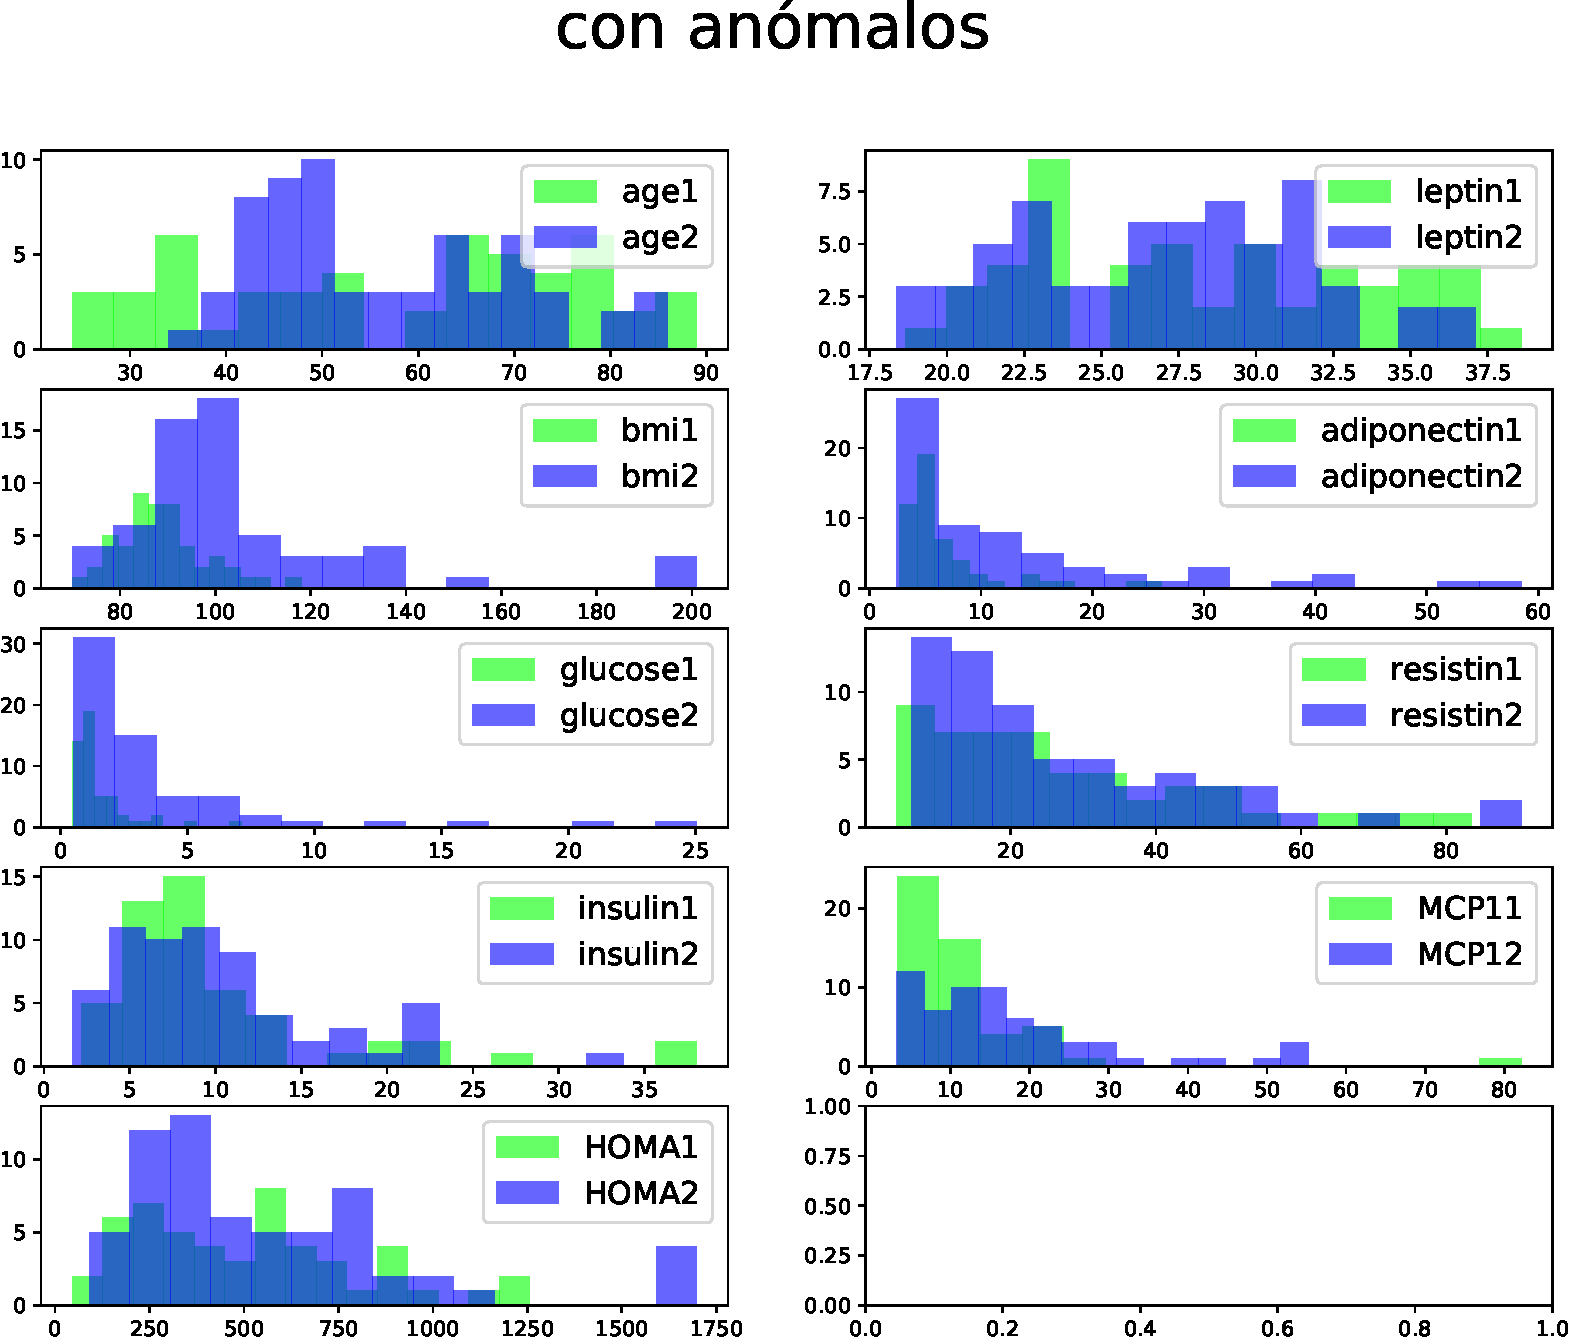
\includegraphics[width = 0.49\linewidth]{../python/images/hist.pdf}
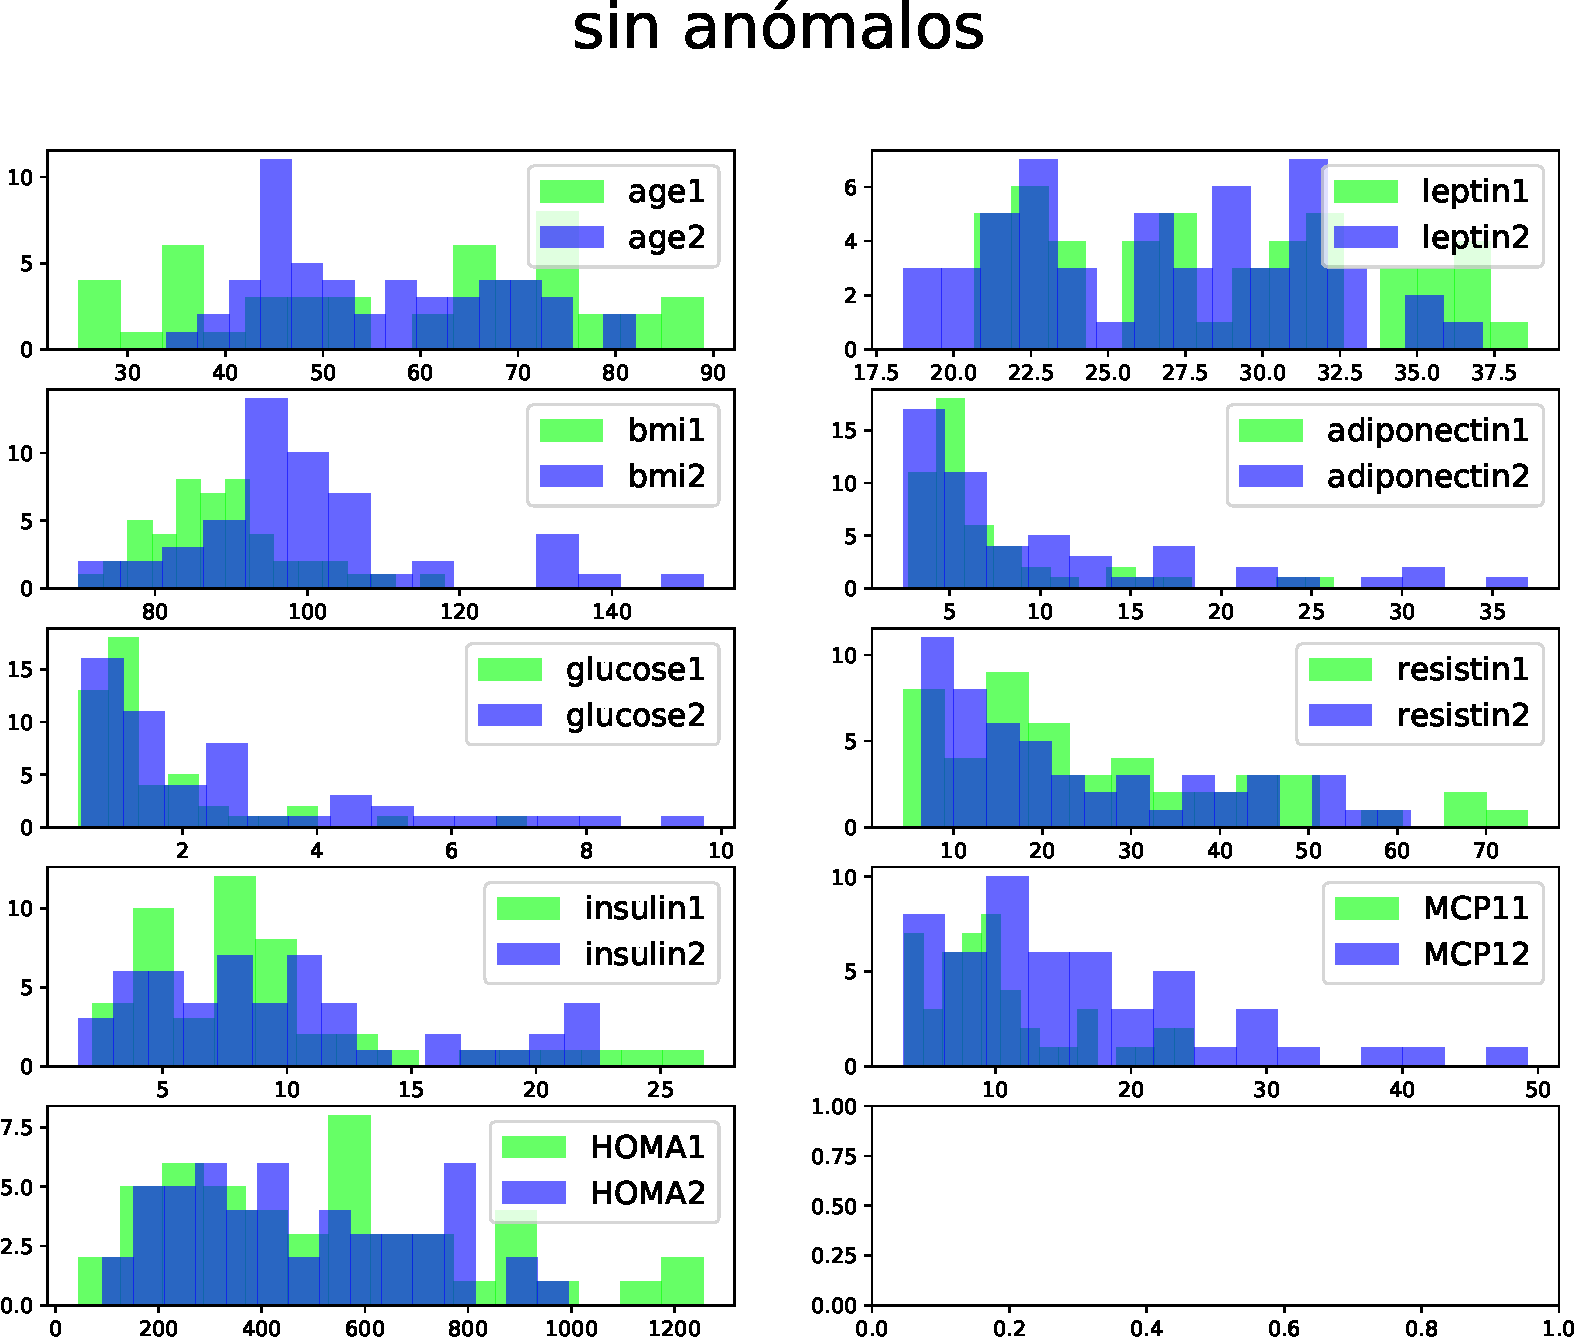
\includegraphics[width = 0.49\linewidth]{../python/images/hist1.pdf}
\caption{Histogramas para datos con y sinanomalias.}
\label{fig:LABEL_NAME}
\end{figure}
\end{document}

